\documentclass[tikz,border=10pt]{standalone}
% Only base TikZ is needed; no extra libraries.
\begin{document}
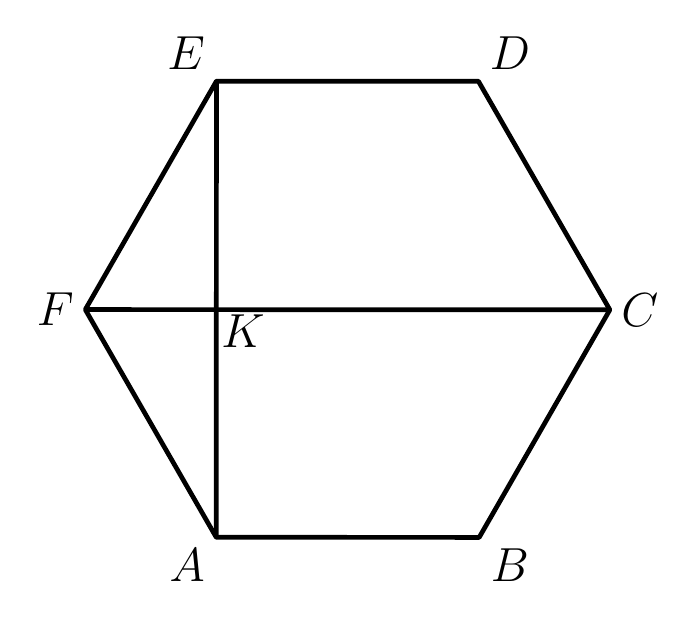
\begin{tikzpicture}[line join=round, line width=1.7pt]
  % Vertices: GES units (1 unit = 100 px) scaled by 2.122 cm per unit (metrics scale 0.02122 cm/px * 100 px)
  \coordinate (E) at (3.122562330688705,-1.3810684735494476);
  \coordinate (D) at (6.449700607395046,-1.3824643346908907);
  \coordinate (C) at (8.118926565805817,-4.284934274461136);
  \coordinate (B) at (6.459370780677833,-7.17547846460813);
  \coordinate (A) at (3.1201319429028698,-7.174077526820758);
  \coordinate (F) at (1.456962844433415,-4.282139327118708);
  \coordinate (K) at (3.1213449280963133,-4.282837598750929);

  % Hexagon outline
  \draw (E) -- (D) -- (C) -- (B) -- (A) -- (F) -- cycle;

  % Interior segments through K
  \draw (F) -- (C);
  \draw (E) -- (A);

  % Labels
  \node[above left] at (E) {\fontsize{17}{20.4}\selectfont $E$};
  \node[above right] at (D) {\fontsize{17}{20.4}\selectfont $D$};
  \node[right] at (C) {\fontsize{17}{20.4}\selectfont $C$};
  \node[below right] at (B) {\fontsize{17}{20.4}\selectfont $B$};
  \node[below left] at (A) {\fontsize{17}{20.4}\selectfont $A$};
  \node[left] at (F) {\fontsize{17}{20.4}\selectfont $F$};
  \node[below right, inner sep=1pt] at (K) {\fontsize{17}{20.4}\selectfont $K$};
\end{tikzpicture}
\end{document}